\documentclass[12pt]{article}

\usepackage[UTF8]{ctex}
\usepackage{appendix}
\usepackage{enumerate}
\usepackage{amsmath}
\usepackage{graphicx}
\graphicspath{{picture/}}
\usepackage{cite}
\usepackage{array}
\usepackage{caption}
\usepackage{bigstrut}
\usepackage{geometry}
\geometry{left =2.5 cm,right=2.5cm,top=2.5cm,bottom=2.5cm}
\usepackage{multirow}
\usepackage{lastpage}
\usepackage{longtable}
\usepackage{listings}
  \usepackage{textcomp} % 必须加上,否则报错
  \usepackage[framed,numbered,autolinebreaks,useliterate]{mcode}    % 添加matlab代码宏
  \usepackage{xcolor}
  \lstset{
  language=Matlab,  %代码语言使用的是matlab
  rulesepcolor=\color{red!20!green!20!blue!20},%代码块边框为淡青色
  keywordstyle=\color{blue!90}\bfseries, %代码关键字的颜色为蓝色,粗体
    numbers=left, % 显示行号
    numberstyle=\tiny,    % 行号字体
   commentstyle=\color[RGB]{0,130,0},    % 设置代码注释的颜色
  showstringspaces=false,%不显示代码字符串中间的空格标记
  stringstyle=\ttfamily, % 代码字符串的特殊格式
  breaklines=true, %对过长的代码自动换行
  extendedchars=false,  %解决代码跨页时,章节标题,页眉等汉字不显示的问题
  escapeinside=``,      % 代码中出现中文必须加上,否则报错
  texcl=true,}
  \lstset{breaklines}
\usepackage[section]{placeins}
\usepackage[colorlinks,linkcolor=blue]{hyperref}
\usepackage{titlesec}
\usepackage{titletoc}
\titleformat{\section}{\heiti\zihao{-3}}{\zhnum{section}、}{0.3em}{}
\titleformat{\subsection}{\heiti \fontsize{12pt}{0}}{\thesubsection}{0.3em}{}
\renewcommand\figurename{\heiti\zihao{5} 图}
\renewcommand\tablename{\heiti\zihao{5} 表}
\renewcommand {\thetable} {\thesection{}.\arabic{table}}
\renewcommand {\thefigure} {\thesection{}.\arabic{figure}}
\renewcommand {\theequation} {\thesection{}.\arabic{equation}}
\date{}
\geometry{a4paper,scale=0.8}
\begin{document}%文档从这里开始。
\captionsetup{labelformat=default,labelsep=space}
\numberwithin{footnote}{section}
\renewcommand\refname{参考文献}
\renewcommand\appendix{\setcounter{secnumdepth}{0}}
\renewcommand\abstractname{摘要}
\begin{figure}[h]
  \centering
  \includegraphics[width=.6\textwidth]{logo}
\end{figure}
\thispagestyle{empty}
\begin{center}
\begin{songti}
\zihao{0}\textbf{电子信息工程课程设计}\\
\zihao{-0}\textbf{心电信号采集与分析}\\
\zihao{-0}\textbf{实验报告}\\\ \\\
\zihao{3}
\\ \
\renewcommand\arraystretch{1.5}
\begin{tabular}{p{1.8cm}<{\centering} p{0.2cm}<{\centering} p{3.5cm}<{\centering} p{1.5cm}<{\centering} p{0.2cm}<{\centering} p{3.5cm}<{\centering}}
课程&\textbf{:}&\multicolumn{4}{c}{\kaishu{电子信息工程课程设计}}\\\cline{3-6}
教师&\textbf{:}&\multicolumn{4}{c}{\kaishu{王志华}}\\\cline{3-6}
组号&\textbf{:}&\multicolumn{4}{c}{\kaishu{第12组}}\\\cline{3-6}
作者&\textbf{:}&\kaishu{许晓明}&学号&\textbf{:}&\kaishu{9161040G0734}\\\cline{3-3}\cline{6-6}
同组人&\textbf{:}&\kaishu{朱泳庚} &学号&\textbf{:}&\kaishu{9161040G0740}\\\cline{3-3}\cline{6-6}
\end{tabular}

\begin{table}[b]
  \centering
\number\year\ 年\ \number\month月
\end{table}

\end{songti}
\end{center}

\newpage
\zihao{-4}
\newpage
\setcounter{page}{1}
\pagenumbering{Roman}
\renewcommand{\contentsname}{\centerline{目录}}
\tableofcontents
\newpage
\setcounter{page}{1}


\setcounter{page}{1}
\pagenumbering{arabic}
\section{设计目的}
\setcounter{table}{0}\setcounter{figure}{0}\setcounter{equation}{0}
通过对心电信号的采集、分析与处理,得出被监测人的心电的有关参数。
\section{设计要求}
\setcounter{table}{0}\setcounter{figure}{0}\setcounter{equation}{0}
\subsection{基本要求}
\begin{enumerate}
 \item  熟悉信号采集工作原理
  \item 利用任意信号发生器产生心电信号;
\item 运用DSP数据采集实验装置采集心电信号,并将采集的数据送到计算机中存储;
\item 利用Matlab编程对心电信号进行处理,显示出心电图,并得出相关心电参数;
\item 撰写课程设计报告。
\end{enumerate}
\subsection{提高要求}
\begin{enumerate}
  \item 修改DSP程序,采用实验装置采集正弦信号并进行处理,在LCD上显示信号频率、幅度等信息;
  \item 修改DSP程序,在实验装置上分析、处理心电信号,得出相关心电参数,并在LCD显示处理结果。
\end{enumerate}
\section{设计内容与步骤}
\setcounter{table}{0}\setcounter{figure}{0}\setcounter{equation}{0}
\subsection{产生心电信号}
如图\ref{xdxh}
所示,心电信号由信号发生器产生,将信号发生器的输出连接到的C2000DSP实验箱的INPUT1端口。
\begin{figure}[htbp]
  \centering
  \includegraphics[height=4cm]{10}\ \includegraphics[height=4cm]{01}
  \caption{信号发生器产生心电信号}\label{xdxh}
\end{figure}
\subsection{连接示波器}
将DSP实验箱的OUT3端口连接示波器。
\subsection{根据液晶显示屏显示的提示信息进行操作}
接通DSP实验箱电源,根据液晶显示屏显示的提示信息进行操作
\begin{enumerate}
  \item 上电后,首先选择4(AD),按ENTER键确认;
\item 通过数字键选择采样频率(符合那奎斯特采样定理,本次试验中采用300Hz),按 ENTER 键确认;
\item 选择“1”保存,通过主机上的采集软件,可将采集的数据通过 USB 线上传到主机。选则“2”不保存,可通过 DSP 试验箱的 OUT3 接口,通过示波器观察波形,若系统正常,应该能够看到跟信号发生器输出一致的波形,以此来验证电路系统的正确性;
\item 若在 3)选择“1”保存后,主机会提示安装USB驱动,正确安装驱动后,打开主机上的数据采集软件,会出现如图\ref{sjcj}
所示界面;
\begin{figure}[htbp]
  \centering
  \includegraphics[width=.45\textwidth]{20}
  \caption{数据采集软件界面示意图}\label{sjcj}
\end{figure}
\item 点击“start”,开始数据传输,若系统工作正常,Successed Transfers 后会显示“5”,表明收到5个数据包,若显示信息不是5,则将 DSP 试验箱断电,重新开始。
\item 若5)正常,则主机会产生一个数据文件 USB.DAT,这就是ADC采集的数据,共 1024个采样点,每个采样点为12位有效数字,表示为2个字节,高8位在前(其中高4位为 0),低8位在后。
\item 在PC端接收实验箱传输的采样数据,利用编好的MATLAB程序进行数据处理。
\item 观察PC端MATLAB显示结果,逐步调试改进程序。
\item 修改程序并对数据进行分析最后给出健康分析。
\item 重新采集两组数据进行对比试验。两组信号分别为:
\begin{enumerate}[1).]
 \item  2Hz,600Mv
 \item  1Hz,400mV
\end{enumerate}
\end{enumerate}
\section{设计原理}
\setcounter{table}{0}\setcounter{figure}{0}\setcounter{equation}{0}
\subsection{心电信号的分析参照标准}
如图\ref{zcxdt}
所示,心电图的指标正常要求范围是:
\begin{figure}[htbp]
  \centering
  \includegraphics[width=.7\textwidth]{21}
  \caption{正常心电图波形示意图}\label{zcxdt}
\end{figure}
正常窦性心率 60 $-$ 100bpm (对应的RR间期为1s $-$ 0.6s)。
\subsection{MATLAB数据处理原理}
\begin{enumerate}
  \item 实验数据在通过DSP实验箱进行数据采集时会产生电噪声,影响数据分析,故在数据频谱分析前需要进行隔直、归一化与滤波,实验中滤除直流分量可以使用参考语句 data=data-mean(data),滤波采用加凯瑟窗(具体程序见附录)。
\item 心率即心脏在一分钟之内跳动的次数,其产生次数表现在波形上即为一段时间内R峰出现的次数,因而计算心率即要求使用MATLAB编程在处理过的数据中找到所有最大波峰(使用 findpeak 函数),给出所有最大波峰的横纵坐标即时间和电压,对相邻波峰出现的时间间隔取平均数 ,使用公式:
\begin{equation}
  \mbox{心率}=\frac{60}{t}
\end{equation}
\end{enumerate}
\subsection{硬件原理}
DEC2812板的原理框图如图\ref{ylkt}
所示。
\begin{figure}[htbp]
  \centering
  \includegraphics[width=\textwidth]{PPT02}
  \caption{DEC2812板原理框图}\label{ylkt}
\end{figure}\par
数据采集部分组成如图\ref{sjcjkt}
所示。
\begin{figure}[htbp]
  \centering
  \includegraphics[width=\textwidth]{PPT05}
  \caption{数据采集部分框图}\label{sjcjkt}
\end{figure}\par
数据采集结构图如图\ref{sjcjjgt}
所示。
\begin{figure}[htbp]
  \centering
  \includegraphics[width=\textwidth]{PPT06}
  \caption{数据采集结构图}\label{sjcjjgt}
\end{figure}\par
DSP调试仿真系统组成如图\ref{DSPts}
所示。
\begin{figure}[htbp]
  \centering
  \includegraphics[width=\textwidth]{PPT06}
  \caption{DSP调试仿真系统组成}\label{DSPts}
\end{figure}
\section{软件设计}
\setcounter{table}{0}\setcounter{figure}{0}\setcounter{equation}{0}
\subsection{源代码分析}
本实验中涉及到采样与处理的程序文件主要是AD.c;LCD显示的主要文件是LCD.c。LCD.h中主要存放字模文件。\par
分析AD.C的函数,其中,
\lstset{
language=C,
basicstyle=\tt,
    %行号
    numbers=left,
    rulesepcolor=\color{red!20!green!20!blue!20},
    escapeinside=``,
    xleftmargin=2em,xrightmargin=2em, aboveskip=1em,
    %背景框
    framexleftmargin=1.5mm,
    %frame=shadowbox,
    %背景色
    %backgroundcolor=\color[RGB]{245,245,244},
    %样式
    keywordstyle=\color{blue}\bfseries,
    identifierstyle=\bf,
    numberstyle=\color[RGB]{0,192,192},
    commentstyle=\it\color[RGB]{50,184,16},
    stringstyle=\rmfamily\slshape\color[RGB]{128,0,0},
    %显示空格
    showstringspaces=false,
      breaklines=true,}
\begin{lstlisting}[language=C]
interrupt void adc_isr(void)
{	
	EALLOW;
    GpioDataRegs.GPASET.all = 0xFFFF;
    switch(bz)
	{
    	
		case 33: AD_read();break;
		case 34: AD_DA();break;
        //case 26: FFTZ();break;
        default:break;
    }
\end{lstlisting}
可知每进行一次采样,就进入一次中断服务函数,根据bz的不同进入AD\_read()或AD\_read()。\par
分析AD\_read()函数:\par
\begin{lstlisting}[language=C]
void AD_read()
{	
	result[number]=AdcRegs.ADCRESULT0>>4;
	number++;
	if(number>=1024)
		{
		number=0;
		bz=0;
		read_over=1;
		}
}
\end{lstlisting}
可知AD\_read()函数将采样到的1024个数据赋值给result数组(仅一次);\par分析AD\_DA()函数:
\begin{lstlisting}[language=C]
void AD_DA()
{
	GpioDataRegs.GPBDAT.bit.GPIOB3 = 1;
	xn=AdcRegs.ADCRESULT0;//>>8;
	GpioDataRegs.GPBDAT.bit.GPIOB3 = 0;
	* DAOUT=xn;
}
\end{lstlisting}
可知AD\_DA()函数将采样到的数据直接输出。\par
而在主函数中存在这样一个while循环:
\begin{lstlisting}[language=C]
while(can!=6)
    {
     	fang();
	    if(x != 0)
		{
			can= x;
			a++;
			x = 0;
			
	    }
	}
\end{lstlisting}
此循环是当按下的按键不为6、或无按键按下时的循环。\par
在LCD.C中存在以下函数:
\begin{lstlisting}[language=C]
extern void menu_4(void)
{
    GUILCD_writeCharStr(0x00,0x00,19,FALSE);//正
	GUILCD_writeCharStr(0x00,0x01,20,FALSE);//在
	GUILCD_writeCharStr(0x00,0x02,21,FALSE);//执
	GUILCD_writeCharStr(0x00,0x03,22,FALSE);//行
	GUILCD_writeCharStr(0x02,0x01,37,FALSE);//按
    GUILCD_writeCharStr(0x02,0x02,6,FALSE);//6
    GUILCD_writeCharStr(0x02,0x03,38,FALSE);//返
    GUILCD_writeCharStr(0x02,0x04,39,FALSE);//回
    GUILCD_writeCharStr(0x02,0x05,40,FALSE);//主
    GUILCD_writeCharStr(0x02,0x06,41,FALSE);//界
    GUILCD_writeCharStr(0x02,0x07,42,FALSE);//面
}
\end{lstlisting}
此函数在while(can!=6)循环之前调用,说明对while(can!=6)的作用判断无误。
\subsection{信号处理}
\subsubsection{参数计算}
\paragraph{幅度}
将采样得到的最大值与最小值相减可得到幅度情况,但由于采样得到值并不完全等同于幅度值,取两值验证后有如表
的关系。
\begin{table}[htbp]
  \centering
\begin{tabular}{|c|c|}
  \hline
  输入值(mv)&计算值
  \\
  \hline
 500 &36.4
  \\
  \hline
  200&15
  \\
  \hline
\end{tabular}
\end{table}\par
于是,利用待定系数法构造二元一次方程,修改计算公式为:
\begin{equation}
  \mbox{幅度}=(max-min)\times 14.01869-10.2804
\end{equation}
\paragraph{频率}
计算频率时,设定一阈值:$k\times (max-min)+min$,其中k为一小于1的数,用于判断周期,如图\ref{jsff}
所示,当两次出现当前点小于阈值且下一点大于等于阈值时,认为经过了一个周期。将计数的结果换算得到频率。
\begin{figure}[htbp]
  \centering
  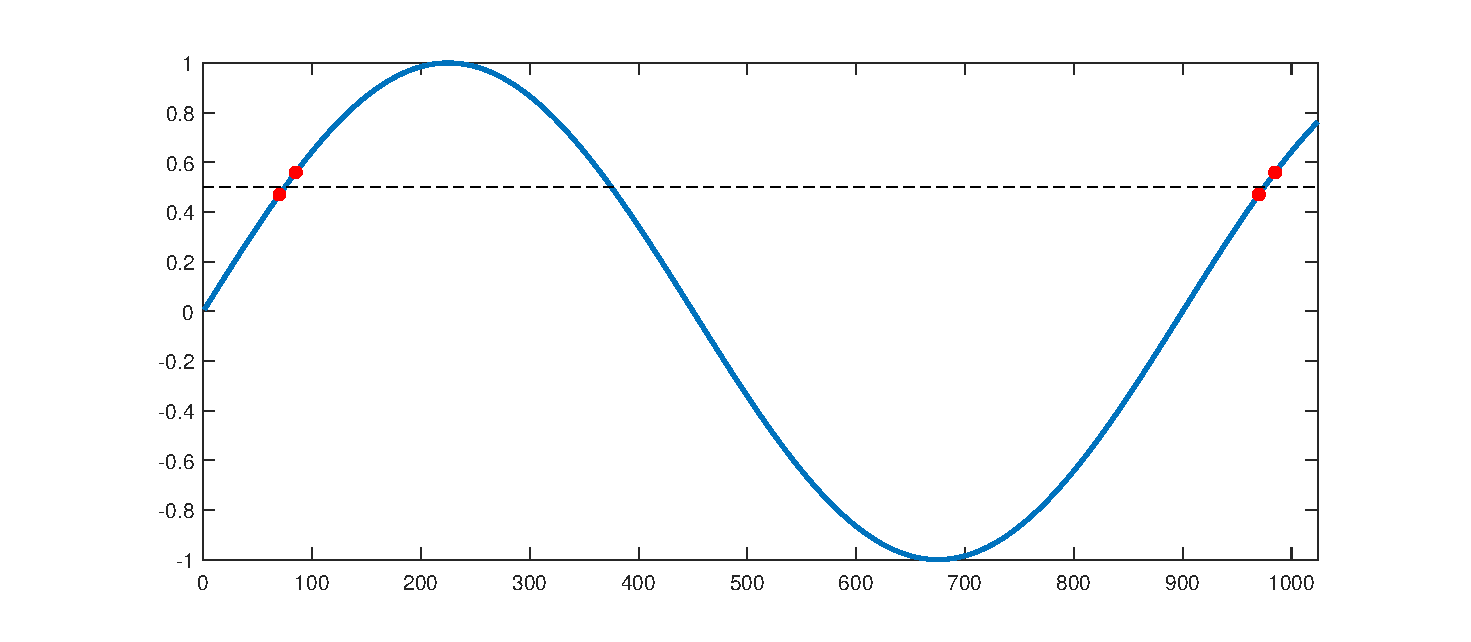
\includegraphics[width=.8\textwidth]{untitled}
  \caption{计算方法示意图}\label{jsff}
\end{figure}
\subsubsection{数据显示}
在LCD.C中存在函数:
\begin{lstlisting}[language=C]
extern void GUILCD_writeCharStr(unsigned int Row, unsigned int Column, unsigned int location ,unsigned short fanxian)
{
//	unsigned int ii1,ii4;
//	ii4 = 0;
	//ii1 = *cString;
	//while(ii1 != 0)				/* 判断字符串是否结束 */
	{
		wr_hex(location,Row*0x10,Column*2,fanxian);	/* 写汉字 */
		//Column++;				/* 列位置+1 */
		//ii4++;
		//ii1 = *(cString + ii4);		/* 读字符串内的值 */
	}
}
\end{lstlisting}
在AD.C中调用此函数,可以实现数据显示。
\subsection{代码实现}
\subsubsection{基于数据存储的代码实现}
由于在AD\_read()中,数据被存储到了result数组中,对result数组进行处理可以实现求参数。考虑到噪声产生的误差,先对数组进行五点均值滤波,其中,数据处理的代码如下:
\begin{lstlisting}[language=C]
void result_calculate()
{
		    int i;
			int k;
			//滤波
for(i=0;i<=1019;i++)
{
result_filter[i]=result[i]+result[i+1]+...
result[i+2]+result[i+3]+result[i+4];
result_filter[i]=result_filter[i]/5;
}

		    result_max = result[0];
			result_min = result[0];


for(k=0;k<1024;k++)
{
if(result[k]>result_max)
{
result_max = result[k];
}
if(result[k]<result_min)
{
result_min = result[k];
}
					
}
threshold=result_min+(result_max-result_min)*0.6;
for(i=0;i<1019;i++)
{
if(	result[i]<threshold && result[i+1]>=threshold)
{interval_result=i-last_i;
last_i=i;
measure_f=adfreq_last/interval_result;}
}
}
\end{lstlisting}
在while(can!=6)中修改的内容如下:
\begin{lstlisting}[language=C]
while(can!=6)
    {
 if(count_display == 0)
            {
                count_display = 20;
	read_over=0;
//	bz = 33;
               AD_read();
               result_calculate();
	change_result=(result_max - result_min)*14.01869-10.2804;

GUILCD_writeCharStr(0x03,0x02,change_result / 10000 % 10,FALSE);
GUILCD_writeCharStr(0x03,0x03,change_result / 1000 % 10,FALSE);
GUILCD_writeCharStr(0x03,0x04,change_result / 100 % 10,FALSE);
GUILCD_writeCharStr(0x03,0x05,change_result / 10 % 10,FALSE);
GUILCD_writeCharStr(0x03,0x06,change_result % 10,FALSE);


GUILCD_writeCharStr(0x05,0x02,result_max / 1000 % 10,FALSE);
GUILCD_writeCharStr(0x05,0x03,result_max / 100 % 10,FALSE);
GUILCD_writeCharStr(0x05,0x04,result_max / 10 % 10,FALSE);
GUILCD_writeCharStr(0x05,0x05,result_max % 10,FALSE);

GUILCD_writeCharStr(0x06,0x02,threshold / 1000 % 10,FALSE);
GUILCD_writeCharStr(0x06,0x03,threshold / 100 % 10,FALSE);
GUILCD_writeCharStr(0x06,0x04,threshold / 10 % 10,FALSE);
GUILCD_writeCharStr(0x06,0x05,threshold % 10,FALSE);

GUILCD_writeCharStr(0x07,0x02,measure_f / 1000000 % 10,FALSE);
GUILCD_writeCharStr(0x07,0x03,measure_f / 100000 % 10,FALSE);
GUILCD_writeCharStr(0x07,0x04,measure_f / 10000 % 10,FALSE);
GUILCD_writeCharStr(0x07,0x05,measure_f / 1000 % 10,FALSE);
GUILCD_writeCharStr(0x07,0x06,measure_f / 1000 %10,FALSE);
GUILCD_writeCharStr(0x07,0x08,measure_f / 10 % 10,FALSE);
GUILCD_writeCharStr(0x07,0x09,measure_f % 10,FALSE);
            }
\end{lstlisting}
\subsubsection{基于实时处理的代码实现}
当选择不保存,数据在AD\_DA()实时处理,由于是实时处理,此时将无法实现去噪,对应的代码如下:
\begin{lstlisting}[language=C]
void AD_DA()
{
	GpioDataRegs.GPBDAT.bit.GPIOB3 = 1;
	xn=AdcRegs.ADCRESULT0;
	result=AdcRegs.ADCRESULT0>>4;
	GpioDataRegs.GPBDAT.bit.GPIOB3 = 0;
	* DAOUT=xn;
	if (result_max<result) result_max=result;
	if (result_min>result) result_min=result;

	/*************测频率***************/
	result_threshold=result_min+(result_max-result_min)*0.8;
	if ( last_result < result_threshold && result>=result_threshold )
	{
		flag_result++;
		if(flag_result>10)
		{
			flag_result=1;
			result_max=result_threshold;
			result_min=result_threshold;
		}
		Freq = adfreq_last*100/Freq_time;
		Freq_time = 1;
	}
	else{Freq_time++;}
	last_result = result;
}
\end{lstlisting}
在while(can!=6)中,修改代码为:

\begin{lstlisting}[language=C]
while(can!=6)
    {
     	fang();
	    if(x != 0)
		{
			can= x;
			a++;
			x = 0;		
	    }
		change_result =( (result_max - result_min)*14.01869-10.2804);
		
		GUILCD_writeCharStr(0x04,0x04,result_max/10%10, FALSE);
		GUILCD_writeCharStr(0x04,0x03,result_max/100%10, FALSE);
		GUILCD_writeCharStr(0x04,0x02,result_max/1000%10, FALSE);
		GUILCD_writeCharStr(0x04,0x01,result_max/10000%10, FALSE);

		GUILCD_writeCharStr(0x06, 0x05, measure_f%10, FALSE);
		GUILCD_writeCharStr(0x06, 0x03, measure_f/10%10, FALSE);
		GUILCD_writeCharStr(0x06, 0x02, measure_f/100%10, FALSE);
		GUILCD_writeCharStr(0x06, 0x01, measure_f/1000%10, FALSE);

		GUILCD_writeCharStr(0x03, 0x05, change_result%10, FALSE);
		GUILCD_writeCharStr(0x03, 0x03, change_result/10%10, FALSE);
		GUILCD_writeCharStr(0x03, 0x02, change_result/100%10, FALSE);
		GUILCD_writeCharStr(0x03, 0x01, change_result/1000%10, FALSE);

		GUILCD_writeCharStr(0x05, 0x04,  result_threshold/10%10, FALSE);
		GUILCD_writeCharStr(0x05, 0x03,  result_threshold/100%10, FALSE);
		GUILCD_writeCharStr(0x05, 0x02,  result_threshold/1000%10, FALSE);
		GUILCD_writeCharStr(0x05, 0x01,  result_threshold/10000%10, FALSE);
	}
\end{lstlisting}
\section{实验结果}
\setcounter{table}{0}\setcounter{figure}{0}\setcounter{equation}{0}
\subsection{基于数据存储的代码的结果}\label{jysjccdjg}
基于数据存储的代码,其结果见图\ref{sjccjg}
。\par 其中,第一行为定度后的幅度值、第二行为result数组的最大值、第三行为根据最大值得出的阈值、第四行为计算出的频率值。
\begin{figure}[htbp]
  \centering
  \begin{tabular}{cc}
  \includegraphics[height=3cm]{18}&\includegraphics[height=3cm]{17}\\
  信号源输入(a)&LCD显示结果(a)\\
  \ &\ \\
    \includegraphics[height=3cm]{19}&\includegraphics[height=3cm]{14}\\
  信号源输入(b)&LCD显示结果(b)\\
  \end{tabular}
  \caption{基于数据存储的代码的结果}\label{sjccjg}
\end{figure}\par
从中可以看出,幅度测量结果大致无误,但频率计算结果不正确。进一步测试后发现,当幅度输入值调大,系统可以实时更新;但当幅度输入值变小,需要一段时间后,系统才会更新。\par
调试后,发现出现问题的原因是,为了完成实时显示,让AD\_read()不断读取数据,但系统处理数据的速度更不上读取的速度,导致计算出频率值之前,数据已经更新,因此频率值始终为0。\par
由于计算幅度的方案是最大值减最小值再进行定度,当输入变大时,最大、最小值可以立刻更新;但当输入变小时,需要等待整个数组全部更新完毕后,才会出现新的“最大值”、“最小值”。
\subsection{基于实时处理的代码的结果}
基于实时处理的代码,其结果见图\ref{sscljg}。\par
同样,第一行为定度后的幅度值、第二行为实时比较得出的最大值(由于直接显示发现超出范围,这里实际上是最大值的1/10)、第三行为根据最大值得出的阈值、第四行为计算出的频率值。
\begin{figure}[htbp]
  \centering
  \begin{tabular}{cc}
  \includegraphics[height=3cm]{04}&\includegraphics[height=3cm]{12}\\
  信号源输入(a)&LCD显示结果(a)\\
   \ &\ \\
    \includegraphics[height=3cm]{05}&\includegraphics[height=3cm]{06}\\
  信号源输入(b)&LCD显示结果(b)\\
   \ &\ \\
      \includegraphics[height=3cm]{07}&\includegraphics[height=3cm]{11}\\
  信号源输入(c)&LCD显示结果(c)\\
   \ &\ \\
        \includegraphics[height=3cm]{15}&\includegraphics[height=3cm]{16}\\
  信号源输入(d)&LCD显示结果(d)\\
  \end{tabular}
  \caption{基于实时处理的代码的结果}\label{sscljg}
\end{figure}\par
从中可以看出,幅度和频率的测量均大致无误。有些许的误差可能是定度时选取的点不合适,以及输出时夹杂的噪声造成的。
\subsection{matlab处理的结果}
利用matlab处理,当输入为1.5Hz时,结果如图\ref{matlabs11}\ $-$\ \ref{matlabs13}
所示。其中,绘制频谱图的目的是确定滤波器的相关参数以实现更好地滤去噪声并观察噪声滤去后的情况。
\begin{figure}[htbp]
  \centering
  \begin{tabular}{c}
  \includegraphics[width=.8\textwidth]{g1}
  \end{tabular}
  \caption{隔直量化后的心电图(时域与频域)}\label{matlabs11}
\end{figure}
\begin{figure}[htbp]
  \centering
  \begin{tabular}{c}
  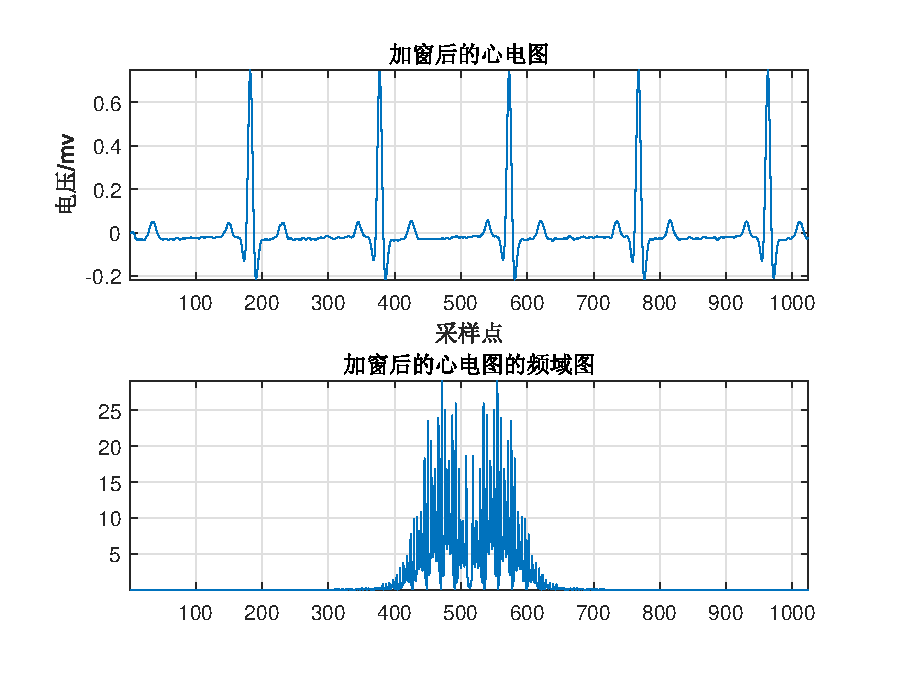
\includegraphics[width=.8\textwidth]{j1}
  \end{tabular}
  \caption{加窗后的心电图(时域与频域)}\label{matlabs12}
\end{figure}
\begin{figure}[htbp]
  \centering
  \begin{tabular}{c}
  \includegraphics[width=.8\textwidth]{x1}
  \end{tabular}
  \caption{matlab输出}\label{matlabs13}
\end{figure}\par
当输入为2Hz时,结果如图\ref{matlabs21}\ $-$\ \ref{matlabs23}
所示。
\begin{figure}[htbp]
  \centering
  \begin{tabular}{c}
  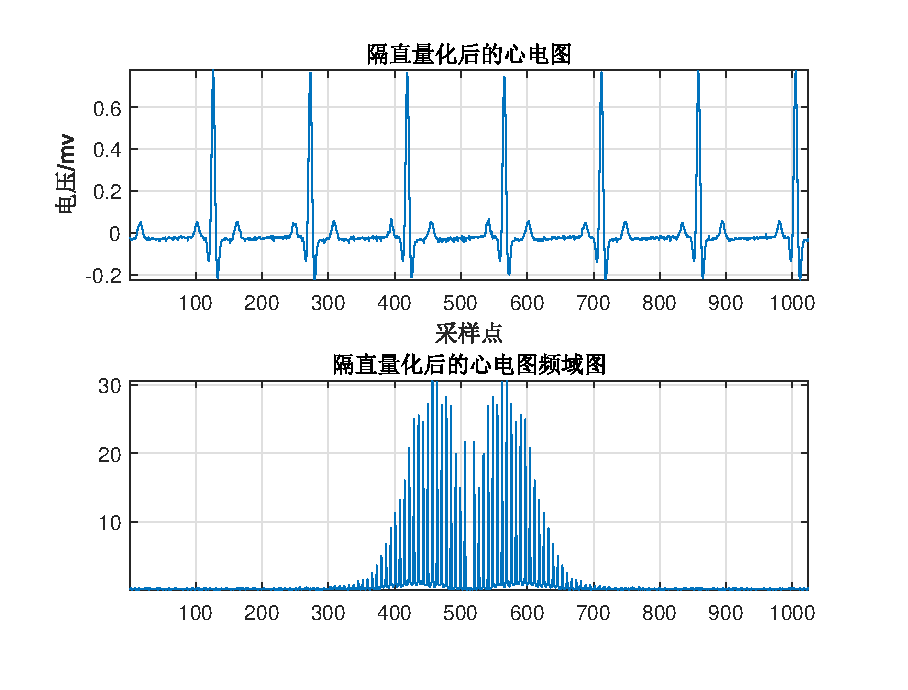
\includegraphics[width=.8\textwidth]{g2}
  \end{tabular}
  \caption{隔直量化后的心电图(时域与频域)}\label{matlabs21}
\end{figure}
\begin{figure}[htbp]
  \centering
  \begin{tabular}{c}
  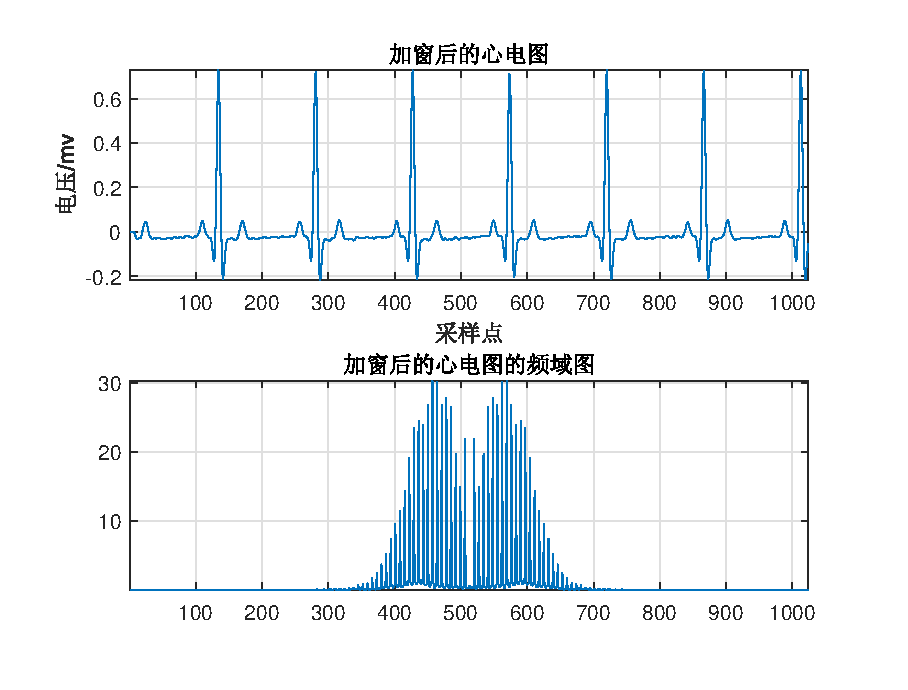
\includegraphics[width=.8\textwidth]{j2}
  \end{tabular}
  \caption{加窗后的心电图(时域与频域)}\label{matlabs22}
\end{figure}
\begin{figure}[htbp]
  \centering
  \begin{tabular}{c}
  \includegraphics[width=.8\textwidth]{x2}
  \end{tabular}
  \caption{matlab输出}\label{matlabs23}
\end{figure}\par
当输入为1Hz时,结果如图\ref{matlabs31}\ $-$\ \ref{matlabs33}
所示。
\begin{figure}[htbp]
  \centering
  \begin{tabular}{c}
  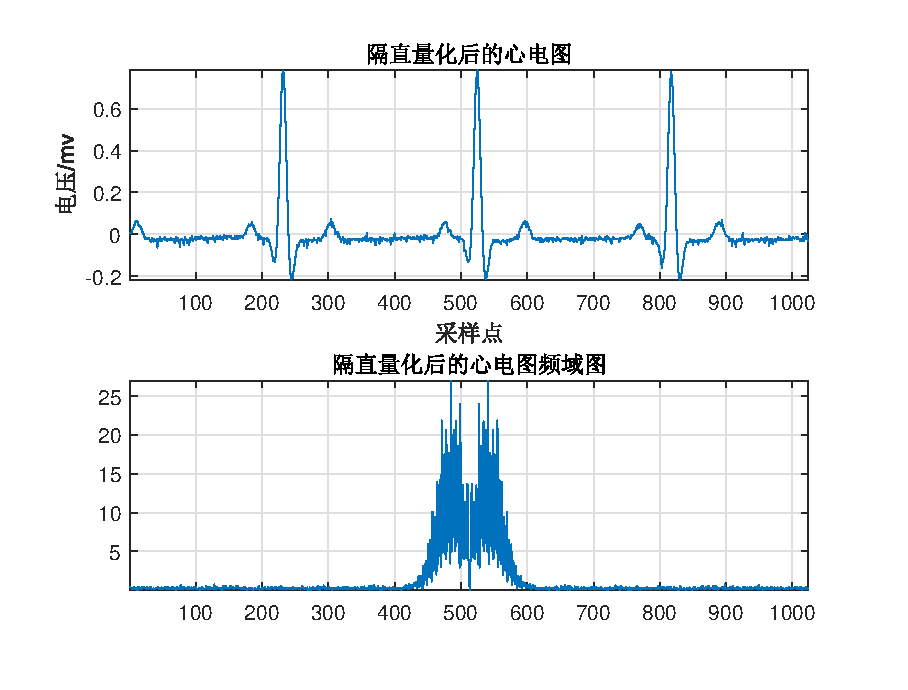
\includegraphics[width=.8\textwidth]{g3}
  \end{tabular}
  \caption{隔直量化后的心电图(时域与频域)}\label{matlabs31}
\end{figure}
\begin{figure}[htbp]
  \centering
  \begin{tabular}{c}
  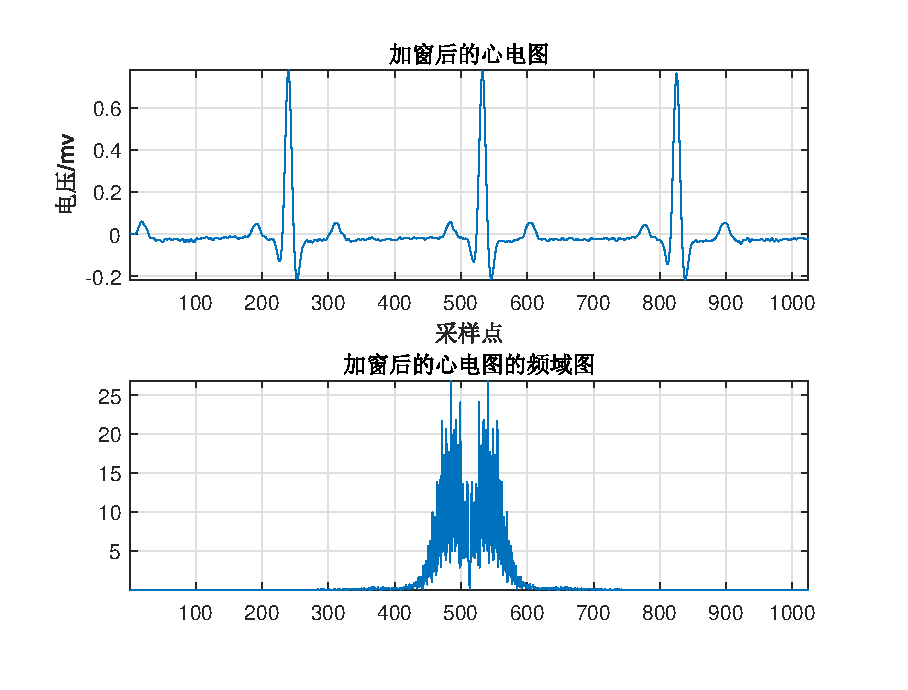
\includegraphics[width=.8\textwidth]{j3}
  \end{tabular}
  \caption{加窗后的心电图(时域与频域)}\label{matlabs32}
\end{figure}
\begin{figure}[htbp]
  \centering
  \begin{tabular}{c}
  \includegraphics[width=.8\textwidth]{x3}
  \end{tabular}
  \caption{matlab输出}\label{matlabs33}
\end{figure}\par
误差情况如表\ref{tab:matlab}
所示。
\begin{table}[htbp]
  \centering
  \caption{MATLAB处理误差情况}
    \begin{tabular}{|c|c|c|c|}
    \hline
    序号 & 心率理论值 & 心率计算值 & 误差 \\
    \hline
    1 & 90 & 92 & 2.222\% \\
    \hline
    2 & 120 & 123 & 2.500\% \\
    \hline
    3 & 60 & 62 & 3.333\% \\
    \hline
    \end{tabular}%
  \label{tab:matlab}%
\end{table}%

\subsection{改进的方向}
从不同的实验方法带来的结果可以看出,实时处理与减小误差有时是矛盾的。\par
因此,为了做到较小的误差,需要进行数据存储与处理。为避免出现\ref{jysjccdjg}的情况,可以设定一个时间t,在t内,数据不更新,直至算出频率。\par
另一方面,计算幅度、频率也并不需要完全用到1024个点,可以减少使用的点数,来加快更新的速度。
\section{实验感想与体会}
\setcounter{table}{0}\setcounter{figure}{0}\setcounter{equation}{0}
在本次实验中,我充分体会到了理论与实际相结合的重要性。\par
事实上,在周一晚,我和马子轩讨论后,已经大致想到了频率的计算方法(阈值判定)。周二当天,我与何超翔共同研读、推敲了程序的运行原理,但在将测频的代码写入程序后,发现显示的频率值始终为零,这使我陷入了困惑,一度毫无进展。后来,何超翔提出可以先尝试测幅度(幅度的测算不需要复杂的计算),并写入了相应的代码。但运行之后的结果仍然是没有变化,我们又陷入了僵局。在周三对代码进行排查后,我们认识到是因为没有给判断的变量赋合适的初值,使得结果始终不更新,在修改完毕后,出现了\ref{jysjccdjg}的结果,即幅度变大可以立刻测出,但幅度变小无法刷新(当时我们还没有想到是由于数组的数据没有全部更新完毕)。 \par
在周三,我们通过调试发现了这个问题,也发现了由于数据的更新使得频率无法测算的问题,但具体如何解决这个问题却没有具体的想法。周四晚,马子轩和陈彪尝试了在AD\_DA()中调用实时采集的数据进行处理,在频率测算上取得了不错的效果。在周五,我也尝试了这种方法,发现不经过滤波,测算得到的频率误差并不大。推测是因为输入的频率不高,信号变化较为平缓,可以忽略噪声带来的影响。事实上,这种方法在测算高于100Hz的频率时会出现较大的误差。\par
本次实验让我体会最深的就是,软件代码在硬件上的运行,尤其是伴随着中断的代码,有时并不是完全按照预想。必须将理论与实践相结合,才有可能实现预期的目标。\par
最后,我要感谢在实验给予我帮助的王志华老师,以及在实验过程中与我一同讨论的马子轩、陈彪、何超翔、李世源等同学。
\section{附录:matlab代码}
\begin{lstlisting}[language=matlab]
%*****************************变量声明***********************************
clc;
clear;
close all;
N=1024;
fs=300;
%******************************采样频率*********************************
Ts=1/fs;
n=0:N-1;
fp=n/N*fs;
%*****************************导入打开文件*******************************
[FileName,PathName] = uigetfile('USB.dat','Select the USB.dat file');
f = fullfile(PathName,filesep,FileName);
fid = fopen(f,'r');
data = fscanf(fid,'%x');
fclose(fid);
%*****************************生成源心电图********************************
data = data(1:2:end)*256 + data(2:2:end);%进制转换
figure(3)
plot(data);
title('原波形图');
grid on;axis tight;
%*******************************隔直、量化生成时域频域图************************
data=data-mean(data);%隔直
dataal=data;
m=max(data);
n=min(data);
data=data/(m-n);%量化
datsgn1 = data;
figure(1)
subplot(2,1,1);
plot(datsgn1);%时域波形
grid on;axis tight;
title('隔直量化后的心电图');
xlabel('采样点');ylabel('电压/mv');
F1=fftshift(fft(datsgn1));
figure(1)
subplot(2,1,2);
plot(abs(F1));
grid on;axis tight;
title('隔直量化后的心电图频域图');
%*****************************滤波、加窗生成时域频域图***************************
%加滤波器
fp=0.05;fc=100;As=80;Ap=1;Fs=300;
wc=2*pi*fc/Fs;
wp=2*pi*fp/Fs;
wd=wc-wp;
beta=0.1102*(As-8.7);
N=ceil((As-7.95)/2.286/wd);
wn=kaiser(N+1,beta);
ws=(wp+wc)/2/pi;
b=fir1(N,ws,wn);
datsgn2=fftfilt(b,data);
F2=fftshift(fft(datsgn2));
figure(2)
subplot(2,1,1);
plot(datsgn2);
grid on;axis tight;
title('加窗后的心电图');
xlabel('采样点');ylabel('电压/mv');
figure(2)
subplot(2,1,2);
plot(abs(F2));
grid on;axis tight;
title('加窗后的心电图的频域图');
 %**************************计算判断显示心率**********************************
[pks,locs] = findpeaks(datsgn2,'MINPEAKDISTANCE',50,'MINPEAKHEIGHT',0.2);
dis=diff(locs);
avrdis=mean(dis);
beat=round(fs/avrdis*60);
display('此人的心率(bpm)为:')
display(num2str(beat))
if beat>=60&&beat<=100
display('正常人的心率在60-100bpm,因此此人心率正常')
else
    if beat<60
display('此人的心率此人心率过低')
    else
    display('此人的心率此人心率过高')
    end
end
\end{lstlisting}
\end{document}
